\section{Ejercicio \#2: Backup de antenas}
\subsection{Introduccion}
El problema es el siguiente: se tiene una red de $n$ antenas, todas conectadas entre si, con una matriz $d = d[1..n, 1..n]$ con las distancias entre todos las antenas. Para ellas se quiere asignar un backup a cada antena, de tal forma que cada antena tenga $k$ vecinos capaces de hacerle backup pero con un limite $b$ de estas. El objetivo es encontrar una asignación de backups que cumpla con estas restricciones, o determinar que no existe tal asignación.

\subsection{Ejemplos}
\subsubsection{Caso con solucion $b=2$}
Supongamos que tenemos 3 antenas en linea recta, con $k=1$, $b=2$ y $D=10$. La matriz de distancias es la siguiente:
\[ d = \begin{bmatrix}
0 & 8 & 16 \\
8 & 0 & 8 \\
16 & 8 & 0
\end{bmatrix} \]
Proponemos nombrar `vecinos' a las antenas que se encuentran a una distancia menor a $D$.

\begin{table}[h]
\centering
\begin{tabular}{|c|c|c|c|}
\hline
\textbf{Antena} & \textbf{Vecinos disponibles} & \textbf{Backup requerido} & \textbf{Opciones} \\
\hline
1 & $\{2\}$ & $k=1$ & Antena 2 \\
\hline
2 & $\{1, 3\}$ & $k=1$ & Antena 1 o 3 \\
\hline
3 & $\{2\}$ & $k=1$ & Antena 2 \\
\hline
\end{tabular}
\caption{Vecinos disponibles para cada antena (distancia $< D=10$). Las antenas 1 y 3 tienen una única opción: elegir antena 2.}
\label{tab:ejemplo_vecinos}
\end{table}

El problema surge inmediatamente: las antenas 1 y 3 no tienen opción --- ambas \textit{deben} elegir a la antena 2 como backup. Esto significa que la antena 2 aparecería en 2 conjuntos de backup (el de 1 y el de 3), llegando a la restricción $b=2$. Luego, la antena 2 puede elegir entre sus vecinos $\{1, 3\}$ para hacer backup.
Sin embargo, si hubieramos tenido $b=1$, entonces la antena 2 no podría ser backup de ambas antenas 1 y 3, y no habría solución posible.
Veamos las soluciones posibles:

\begin{table}[h]
\centering
\begin{tabular}{|c|c|c|}
\hline
\textbf{Antena} & \textbf{Backup asignado} & \textbf{Apariciones como backup} \\
\hline
\multicolumn{3}{|c|}{\textit{Opción A: Antena 2 elige antena 1}} \\
\hline
1 & 2 & Aparece en: $\{2\}$ $\rightarrow$ 1 vez \\
\hline
2 & 1 & Aparece en: $\{1, 3\}$ $\rightarrow$ 2 veces \\
\hline
3 & 2 & Aparece en: $\{1, 3\}$ $\rightarrow$ 2 veces \\
\hline
\multicolumn{3}{|c|}{\textit{Opción B: Antena 2 elige antena 3}} \\
\hline
1 & 2 & Aparece en: $\{1, 3\}$ $\rightarrow$ 2 veces \\
\hline
2 & 3 & Aparece en: $\{2\}$ $\rightarrow$ 1 vez \\
\hline
3 & 2 & Aparece en: $\{1, 2\}$ $\rightarrow$ 2 veces \\
\hline
\end{tabular}
\caption{Ambas opciones son válidas con $b=2$: cada antena aparece en a lo sumo 2 conjuntos de backup.}
\label{tab:ejemplo_soluciones}
\end{table}

\subsubsection{Caso sin solución: $b=1$}

Consideremos el mismo ejemplo anterior pero con $b=1$ en lugar de $b=2$. Las antenas 1 y 3 \textit{deben} elegir a la antena 2 como backup (es la única opción), lo que significa que la antena 2 aparecería en 2 conjuntos de backup. Esto \textbf{viola inmediatamente} la restricción $b=1$ (máximo 1 aparición):

\begin{table}[h]
\centering
\begin{tabular}{|c|c|c|}
\hline
\textbf{Antena} & \textbf{Intento de asignación} & \textbf{Apariciones} \\
\hline
1 & 2 (obligatorio) & --- \\
\hline
2 & 1 o 3 & --- \\
\hline
3 & 2 (obligatorio) & --- \\
\hline
\multicolumn{3}{|c|}{\textbf{Análisis del conflicto}} \\
\hline
\multicolumn{3}{|p{11cm}|}{
La antena 2 aparecería como backup de las antenas 1 y 3, es decir, \textit{2 apariciones}.
Pero $b=1$ exige máximo 1 aparición. No importa lo que elija la antena 2 como su propio backup,
ya ha violado la restricción.
} \\
\hline
\end{tabular}
\caption{Con $b=1$: la antena 2 debe ser backup de ambas 1 y 3 $\Rightarrow$ 2 apariciones $>$ $b=1$ $\Rightarrow$ \textbf{No existe solución}.}
\label{tab:ejemplo_sin_solucion}
\end{table}

\subsection{Modelado del problema}

Para resolver el problema, lo modelamos como un problema de flujo máximo en una red de flujo. La idea es construir una red de flujo tal que encontrar un flujo máximo en esa red corresponda a encontrar una asignación de backups que cumpla con las restricciones del problema.

Nuestra propuesta de modelado es la siguiente:
\begin{itemize}
    \item Creamos un nodo fuente $S$ y un nodo sumidero $T$.
    \item Para cada antena $i$, creamos dos nodos: $A_i$ (representando la antena) y $B_i$ (representando el backup de la antena).
    \item Conectamos el nodo fuente $S$ a cada nodo $A_i$ con una arista de capacidad $k$ (el tamaño requerido del conjunto de backup).
    \item Conectamos cada nodo $B_i$ al nodo sumidero $T$ con una arista de capacidad $b$ (el límite de apariciones como backup).
    \item Para cada par de antenas $(i, j)$ que son vecinos (es decir, $d[i][j] < D$), conectamos el nodo $A_i$ al nodo $B_j$ con una arista de capacidad 1 (representando la posibilidad de que la antena $i$ elija a la antena $j$ como backup).
    \item El objetivo es encontrar un flujo máximo en esta red. Si el flujo máximo es igual a $n \cdot k$ (es decir, cada antena tiene asignados exactamente $k$ backups), entonces existe una solución válida. De lo contrario, no existe tal asignación.
\end{itemize}

\begin{figure}[h]
\centering
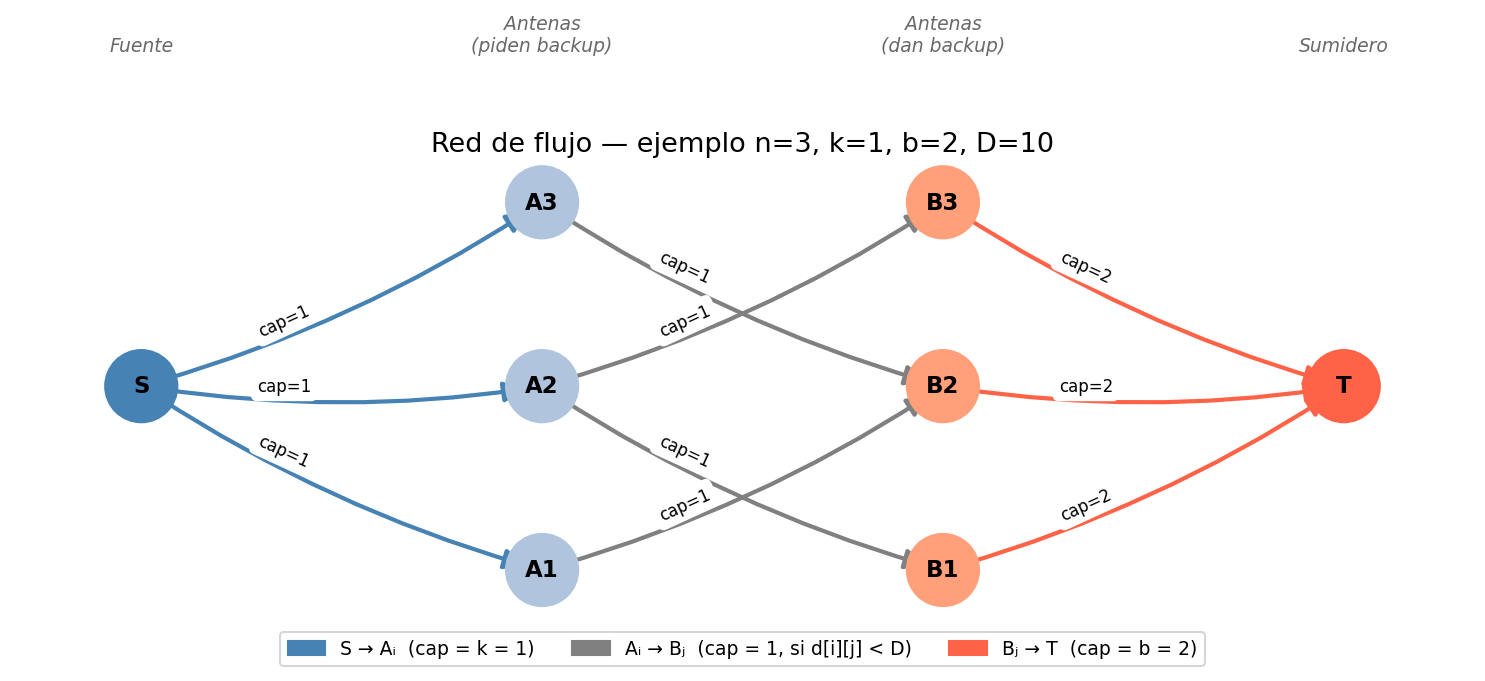
\includegraphics[width=0.9\textwidth]{img/grafico_red.png}
\caption{Red de flujo para el ejemplo con $n=3$, $k=1$, $b=2$, $D=10$. Los nodos $A_i$ piden backup; los nodos $B_j$ lo proveen. El flujo máximo $= n \cdot k = 3$ indica que existe solución. Generado con \texttt{grafico\_red.py}.}
\label{fig:red_flujo}
\end{figure}

\subsection{Diseño de la solución}

\subsubsection{Adaptación al problema de flujo máximo}

La clave del diseño es reconocer que el problema tiene la estructura de una \textbf{asignación bipartita con cuotas}: de un lado están las antenas que \textit{demandan} backups, del otro las antenas que \textit{proveen} backups, y el flujo que pasa por la red representa exactamente qué antena respalda a cuál.

La red se construye con $2n + 2$ nodos organizados en cuatro capas:

\begin{enumerate}
    \item \textbf{Fuente $S$}: inyecta $k$ unidades de flujo hacia cada antena demandante. La capacidad $k$ de la arista $S \to A_i$ fuerza a que cada antena obtenga \textit{exactamente} $k$ backups (ni más, ni menos, dado que el flujo total debe ser $n \cdot k$).
    \item \textbf{Nodos $A_i$ (demanda)}: cada antena $i$ que necesita backup. El flujo que sale de $A_i$ representa qué antenas conforman su conjunto de backup.
    \item \textbf{Nodos $B_j$ (oferta)}: cada antena $j$ en su rol de proveedora de backup. La arista $A_i \to B_j$ existe solo si $d[i][j] < D$, con capacidad 1 (una antena puede aparecer a lo sumo una vez en el backup de cada otra).
    \item \textbf{Sumidero $T$}: absorbe el flujo de todos los $B_j$. La capacidad $b$ de la arista $B_j \to T$ limita cuántos conjuntos de backup distintos puede integrar la antena $j$.
\end{enumerate}

\paragraph{Interpretación de la salida.}
Una vez ejecutado Edmonds-Karp, la respuesta se lee directamente de la red residual:

\begin{itemize}
    \item Si \textbf{flujo máximo $= n \cdot k$}: existe solución. La arista $A_i \to B_j$ está saturada (capacidad residual $= 0$) si y solo si $j$ pertenece al conjunto de backup de $i$.
    \item Si \textbf{flujo máximo $< n \cdot k$}: no existe solución. El corte mínimo certifica que algún subconjunto de antenas no puede obtener suficientes backups respetando el límite $b$.
\end{itemize}

\subsubsection{Pseudocódigo}

\lstinputlisting[
    caption={Pseudocódigo del algoritmo de backup de antenas},
    label={lst:pseudocodigo},
]{code/backup_antenas.pseudo}

\paragraph{Estructuras de datos.}
La red residual se representa como una \textbf{matriz de adyacencia} \texttt{cap[u][v]} de tamaño $(2n+2) \times (2n+2)$, donde \texttt{cap[u][v]} almacena la capacidad residual de $u$ a $v$. Esta elección simplifica la actualización de aristas inversas (siempre existe \texttt{cap[v][u]}) a costa de $O(n^2)$ de memoria, aceptable para los tamaños de instancia esperados.

\subsection{Supuestos}
Los supuestos sobre los que este algoritmo se basa son:

\begin{itemize}
    \item La red es conexa, es decir, existe un camino entre cualquier par de antenas.
    \item Las distancias entre antenas son simétricas, es decir, $d[i][j] = d[j][i]$ para todas las antenas $i$ y $j$.
    \item Ninguna antena puede ser su propio backup.
    \item Las distancias entre antenas no son negativas. 
    \item La matriz de distancias esta completa, incluyendo la diagonal principal (es decir, $d[i][i] = 0$ para todas las antenas $i$).
    \item Los parámetros $k$ y $b$ son enteros no negativos, y $D$ es un número real positivo.
    \item No se considera el posicionamiento en el espacio de las antenas, solo sus distancias mutuas.
\end{itemize}

\subsection{Evaluaciones y resultadoss}

Se ejecutaron 10 casos de prueba sobre el algoritmo implementado. Los casos fueron generados aleatoriamente con semilla fija (para reproducibilidad) mediante el script \texttt{generar\_caso.py}, ubicando las antenas en coordenadas 2D uniformes dentro de un área de $100 \times 100$, con distancias euclídeas. El caso 1 fue construido manualmente. Las mediciones se realizaron en una misma máquina y corresponden al tiempo de ejecución del algoritmo de flujo máximo (sin contar lectura de archivos).

\lstinputlisting[
    caption={Resultados de ejecución sobre los 10 casos de prueba (generado por \texttt{ejecutar\_casos.py})},
    label={lst:mediciones},
]{resultados/flujo/resultados.txt}

\paragraph{Observaciones.}
\begin{itemize}
    \item \textbf{caso\_b\_menor\_k}: con $b=2 < k=3$, la capacidad total de la red ($n \cdot b = 16$) es menor a la demanda total ($n \cdot k = 24$), por lo que es imposible estructuralmente, independientemente de las distancias.
    \item \textbf{caso\_d\_chico vs.\ caso\_d\_amplio}: mismo layout geométrico (misma semilla), distinto $D$. Ambos resultan sin solución porque con $n=10$ antenas dispersas en $100 \times 100$, $D=45$ no garantiza 3 vecinos por antena en esa distribución particular.
    \item \textbf{Tiempo de ejecución}: el tiempo crece con $n$, consistente con la complejidad $O(V \cdot E^2)$ de Edmonds-Karp. El caso \texttt{caso\_grande\_imposible} ($n=50$) tarda casi lo mismo que \texttt{caso\_grande} porque Edmonds-Karp igualmente explora la red antes de concluir que no hay solución.
\end{itemize}